% move all configuration stuff into includes file so we can focus on the content
\documentclass[aspectratio=169,hyperref={pdfpagelabels=false,colorlinks=true,linkcolor=white,urlcolor=blue},t]{beamer}

%%%%%%%%%%%%%%%%%%%%%%%%%%%%%%%%%%%%%%%%%%%%%%%%%%%%%%%%%%%%%%%%%%%%%%%%%%%%%%%%%%
%%%%%%%%%%%%%%%%%%%%%%%%%%%%%%%%%%%%%%%%%%%%%%%%%%%%%%%%%%%%%%%%%%%%%%%%%%%%%%%%%%
% packages
\usepackage{pict2e}
\usepackage{epic}
\usepackage{amsmath,amsfonts,amssymb}
\usepackage{units}
\usepackage{fancybox}
\usepackage[absolute,overlay]{textpos} 
\usepackage{media9} % avi2flv: "C:\Program Files\ffmpeg\bin\ffmpeg.exe" -i TuneFreqFilterbank.avi -b 600k -s 441x324 -r 15 -acodec copy TuneFreqFilterbank.flv
\usepackage{animate}
\usepackage{gensymb}
\usepackage{multirow}
\usepackage{silence}
\usepackage[backend=bibtex,style=ieee]{biblatex}
\AtEveryCitekey{\iffootnote{\tiny}{}}
\addbibresource{references}

%%%%%%%%%%%%%%%%%%%%%%%%%%%%%%%%%%%%%%%%%%%%%%%%%%%%%%%%%%%%%%%%%%%%%%%%%%%%%%%%%%
%%%%%%%%%%%%%%%%%%%%%%%%%%%%%%%%%%%%%%%%%%%%%%%%%%%%%%%%%%%%%%%%%%%%%%%%%%%%%%%%%%
% relative paths
\graphicspath{{graph/}}


%%%%%%%%%%%%%%%%%%%%%%%%%%%%%%%%%%%%%%%%%%%%%%%%%%%%%%%%%%%%%%%%%%%%%%%%%%%%%%%%%%
%%%%%%%%%%%%%%%%%%%%%%%%%%%%%%%%%%%%%%%%%%%%%%%%%%%%%%%%%%%%%%%%%%%%%%%%%%%%%%%%%%
% units
\setlength{\unitlength}{1mm}

%%%%%%%%%%%%%%%%%%%%%%%%%%%%%%%%%%%%%%%%%%%%%%%%%%%%%%%%%%%%%%%%%%%%%%%%%%%%%%%%%%
%%%%%%%%%%%%%%%%%%%%%%%%%%%%%%%%%%%%%%%%%%%%%%%%%%%%%%%%%%%%%%%%%%%%%%%%%%%%%%%%%%
% theme & layout
\usetheme{Frankfurt}
\beamertemplatenavigationsymbolsempty
%\setbeamertemplate{frametitle}[smoothbars theme]
\setbeamertemplate{frametitle}
{
    \begin{beamercolorbox}[ht=1.8em,wd=\paperwidth]{frametitle}
        \vspace{-.1em}%
        \hspace{.2em}{\strut\insertframetitle\strut}
        
        \hspace{.2em}\small\strut\insertframesubtitle\strut
        %\hfill
        %
\includegraphics[height=.8cm,keepaspectratio]{CenterMusicTechnology-solid-2lines-white-CoAtag}
        
    \end{beamercolorbox}
    \begin{textblock*}{100mm}(11.6cm,.7cm)
        \includegraphics[height=.8cm,keepaspectratio]{logo_GTCMT_black}
    \end{textblock*}
}

% set this to ensure bulletpoints without subsections
\usepackage{remreset}
\makeatletter
\@removefromreset{subsection}{section}
\makeatother
\setcounter{subsection}{1}

%---------------------------------------------------------------------------------
% appearance
\setbeamercolor{structure}{fg=gtgold}
\setbeamercovered{transparent} %invisible
\setbeamercolor{bibliography entry author}{fg=black}
\setbeamercolor*{bibliography entry title}{fg=black}
\setbeamercolor*{bibliography entry note}{fg=black}

%\usepackage{pgfpages}
%\setbeameroption{show notes}
%\setbeameroption{show notes on second screen=right}
%---------------------------------------------------------------------------------
% fontsize
\let\Tiny=\tiny

%%%%%%%%%%%%%%%%%%%%%%%%%%%%%%%%%%%%%%%%%%%%%%%%%%%%%%%%%%%%%%%%%%%%%%%%%%%%%%%%%%
%%%%%%%%%%%%%%%%%%%%%%%%%%%%%%%%%%%%%%%%%%%%%%%%%%%%%%%%%%%%%%%%%%%%%%%%%%%%%%%%%%
% warnings
\pdfsuppresswarningpagegroup=1
\WarningFilter{biblatex}{Patching footnotes failed}
\WarningFilter{latexfont}{Font shape}
\WarningFilter{latexfont}{Some font shapes}
\WarningFilter{gensymb}{Not defining}


%%%%%%%%%%%%%%%%%%%%%%%%%%%%%%%%%%%%%%%%%%%%%%%%%%%%%%%%%%%%%%%%%%%%%%%%%%%%%%%%%%
%%%%%%%%%%%%%%%%%%%%%%%%%%%%%%%%%%%%%%%%%%%%%%%%%%%%%%%%%%%%%%%%%%%%%%%%%%%%%%%%%%
% title information
\title[]{Introduction to Audio Content Analysis}   
\author[alexander lerch]{alexander lerch} 
%\institute{~}
%\date[Alexander Lerch]{}
\titlegraphic{\vspace{-16mm}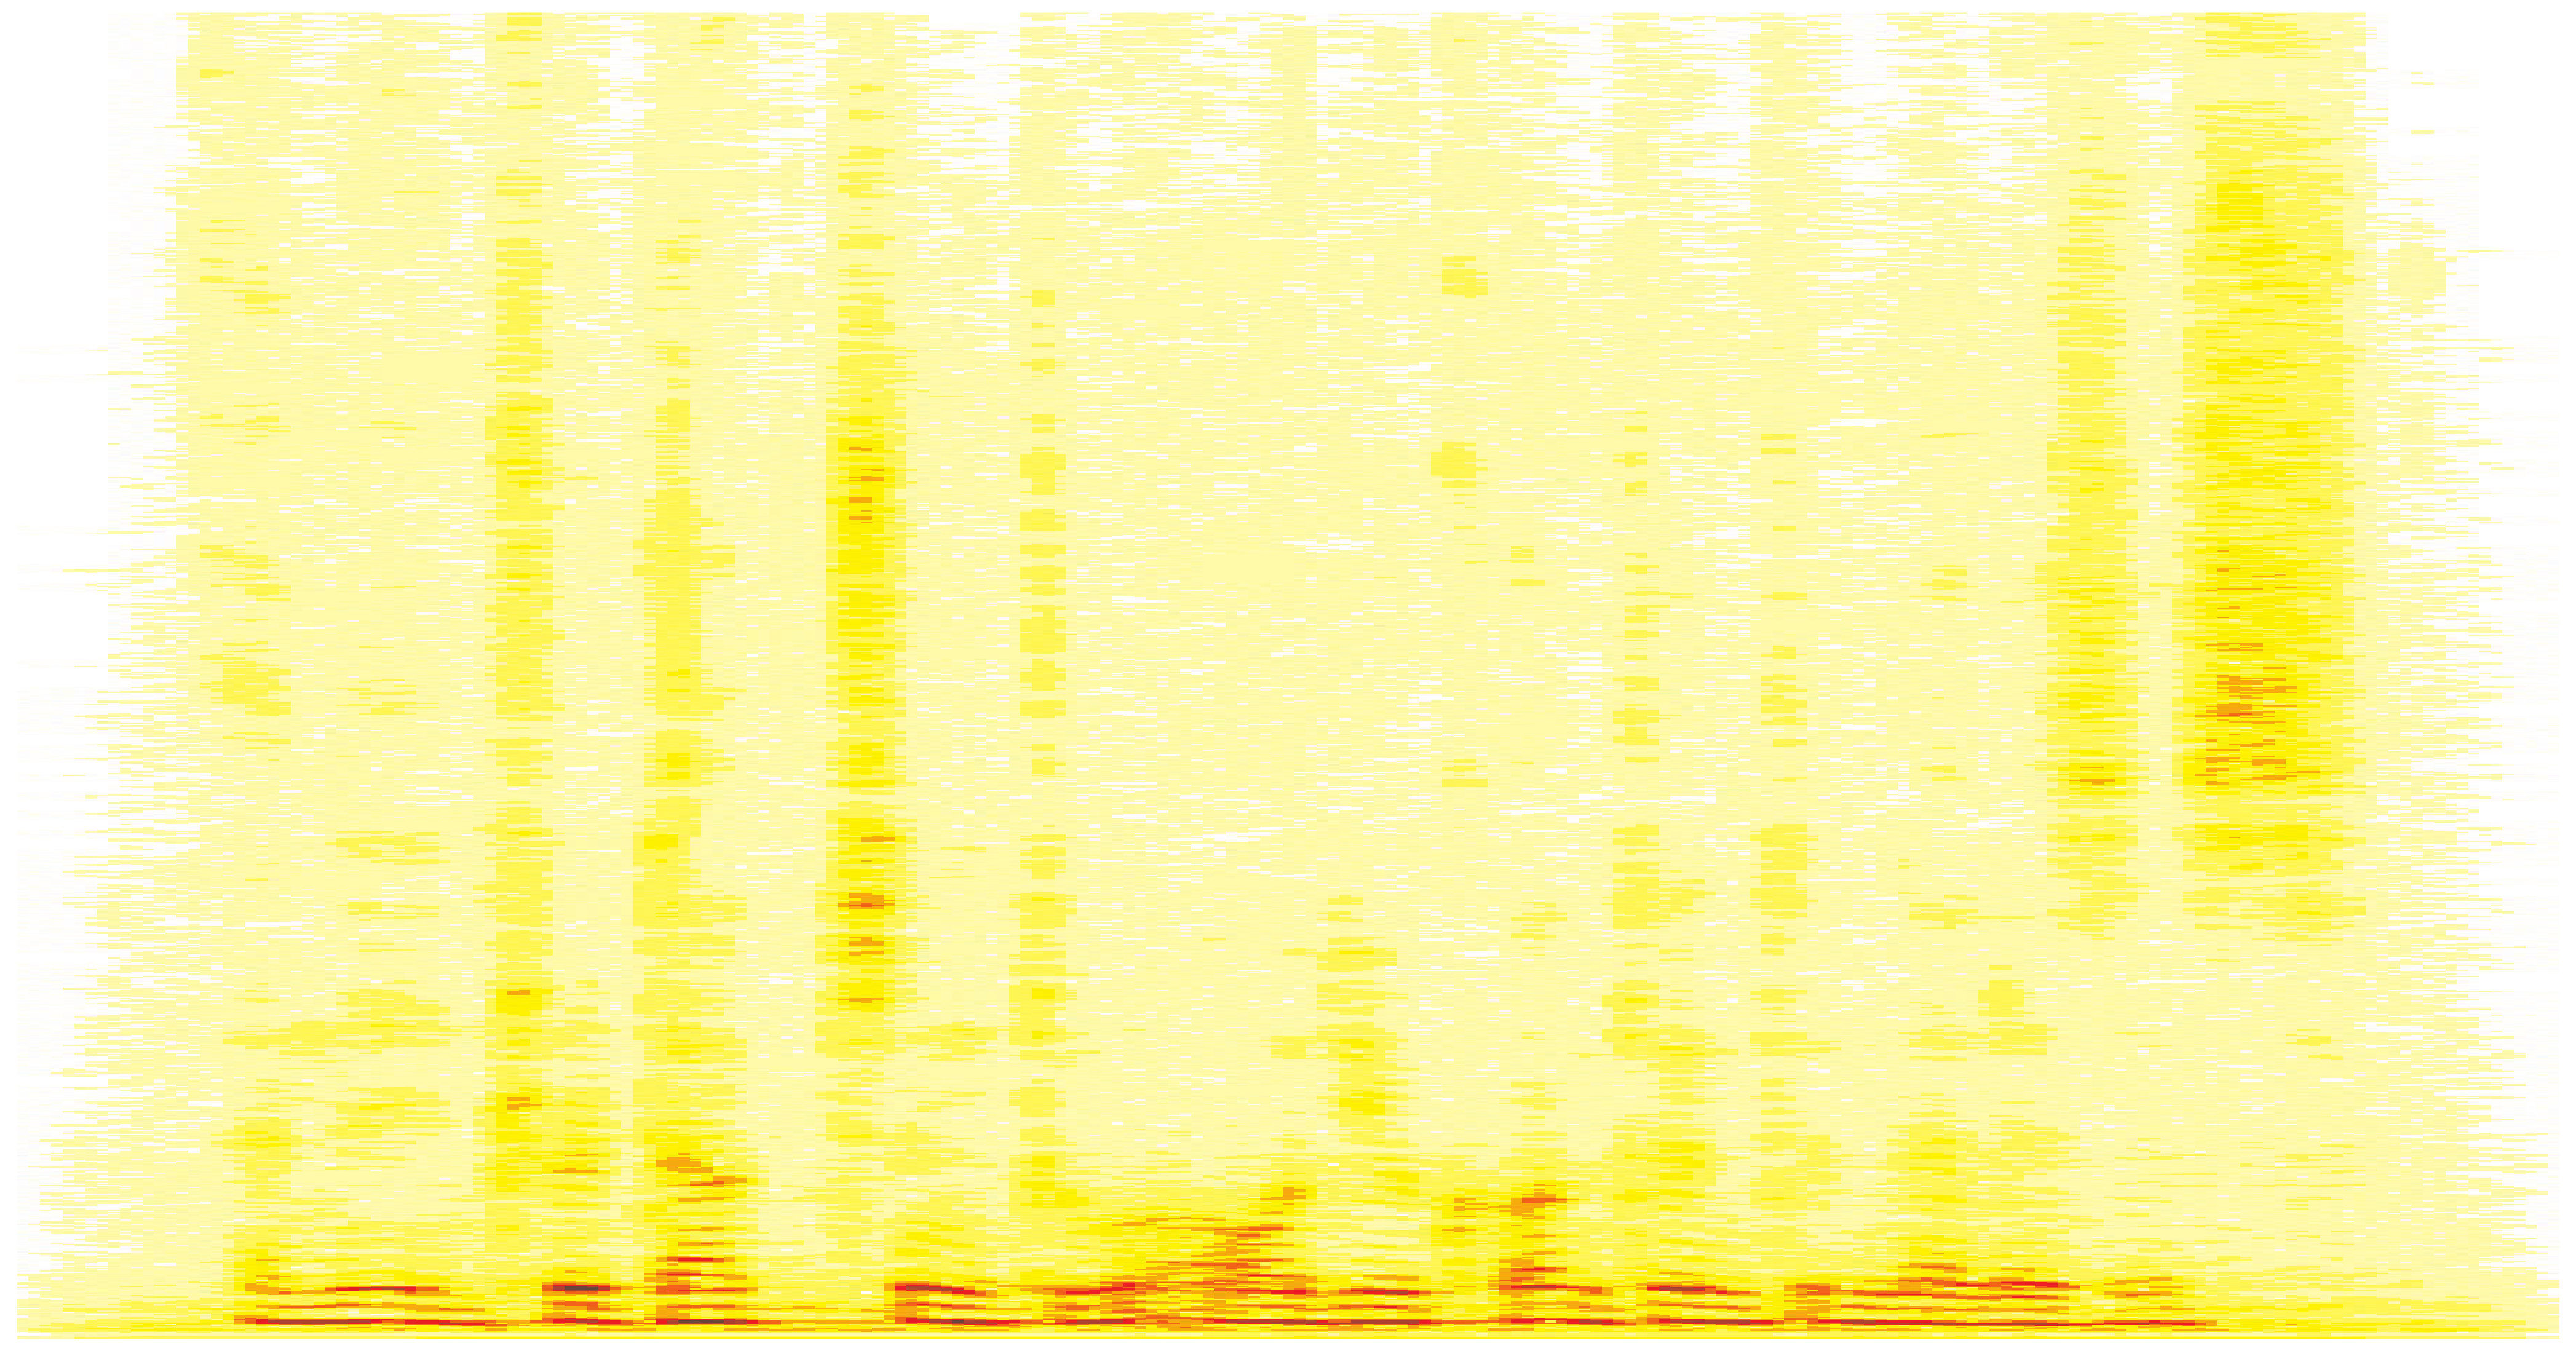
\includegraphics[width=\textwidth,height=3cm]{title}}

%%%%%%%%%%%%%%%%%%%%%%%%%%%%%%%%%%%%%%%%%%%%%%%%%%%%%%%%%%%%%%%%%%%%%%%%%%%%%%%%%%
%%%%%%%%%%%%%%%%%%%%%%%%%%%%%%%%%%%%%%%%%%%%%%%%%%%%%%%%%%%%%%%%%%%%%%%%%%%%%%%%%%
% colors
\definecolor{gtgold}{HTML}{E0AA0F} %{rgb}{0.88,0.66,1,0.06} [234, 170, 0]/256

%%%%%%%%%%%%%%%%%%%%%%%%%%%%%%%%%%%%%%%%%%%%%%%%%%%%%%%%%%%%%%%%%%%%%%%%%%%%%%%%%%
%%%%%%%%%%%%%%%%%%%%%%%%%%%%%%%%%%%%%%%%%%%%%%%%%%%%%%%%%%%%%%%%%%%%%%%%%%%%%%%%%%
% math
\DeclareMathOperator*{\argmax}{argmax}
\DeclareMathOperator*{\argmin}{argmin}
\DeclareMathOperator*{\atan}{atan}
\DeclareMathOperator*{\arcsinh}{arcsinh}
\DeclareMathOperator*{\sign}{sign}
\DeclareMathOperator*{\tcdf}{tcdf}
\DeclareMathOperator*{\si}{sinc}
\DeclareMathOperator*{\princarg}{princarg}
\DeclareMathOperator*{\arccosh}{arccosh}
\DeclareMathOperator*{\hwr}{HWR}
\DeclareMathOperator*{\flip}{flip}
\DeclareMathOperator*{\sinc}{sinc}
\DeclareMathOperator*{\floor}{floor}
\newcommand{\e}{{e}}
\newcommand{\jom}{\mathrm{j}\omega}
\newcommand{\jOm}{\mathrm{j}\Omega}
\newcommand   {\mat}[1]    		{\boldsymbol{\uppercase{#1}}}		%bold
\renewcommand {\vec}[1]    		{\boldsymbol{\lowercase{#1}}}		%bold

%%%%%%%%%%%%%%%%%%%%%%%%%%%%%%%%%%%%%%%%%%%%%%%%%%%%%%%%%%%%%%%%%%%%%%%%%%%%%%%%%%
%%%%%%%%%%%%%%%%%%%%%%%%%%%%%%%%%%%%%%%%%%%%%%%%%%%%%%%%%%%%%%%%%%%%%%%%%%%%%%%%%%
% media9
\newcommand{\includeaudio}[1]{{\includemedia[
                        addresource=audio/#1.mp3,
                        width=5mm,
                        height=5mm,
                        activate=onclick,
                        flashvars={
                            source=audio/#1.mp3  
                            &autoPlay=true
                        }]
                        {
\includegraphics[width=5mm, height=5mm]{SpeakerIcon}}
                        {APlayer.swf}}}
\newcommand{\audioautoplay}[1]{{\begin{center}\includemedia[
                            addresource=audio/#1.mp3,
                            width=.1\linewidth,
                            height=.01\linewidth,
                            activate=pageopen,
                            flashvars={
                                source=audio/#1.mp3  
                                &autoPlay=true
                            }]
                            {}
                            {APlayer.swf}\end{center}}}

\newcommand{\includevideo}[1]{{\begin{center}\includemedia[
                        addresource=video/#1.mp4,
                        width=0.8\linewidth,
                        height=0.4\linewidth,
                        activate=onclick,
                        flashvars={
                            source=video/#1.mp4  
                            &autoPlay=true
                        }]
                        {}
                        {VPlayer.swf}\end{center}}}
\newcommand{\videowithmatlab}[1]{{\begin{center}\includemedia[
                        addresource=video/animate#1.mp4,
                        width=0.8\linewidth,
                        height=0.4\linewidth,
                        activate=onclick,
                        flashvars={
                            source=video/animate#1.mp4  
                            &autoPlay=true
                        }]
                        {}
                        {VPlayer.swf}\end{center}\addreference{matlab source: matlab/animate#1.m}}}
                        

%%%%%%%%%%%%%%%%%%%%%%%%%%%%%%%%%%%%%%%%%%%%%%%%%%%%%%%%%%%%%%%%%%%%%%%%%%%%%%%%%%
%%%%%%%%%%%%%%%%%%%%%%%%%%%%%%%%%%%%%%%%%%%%%%%%%%%%%%%%%%%%%%%%%%%%%%%%%%%%%%%%%%
% other commands
\newcommand{\question}[1]{%\vspace{-4mm}
                          \setbeamercovered{invisible}
                          \begin{columns}[T]
                            \column{.8\textwidth}
                                \textbf{#1}
                            \column{.2\textwidth}
                                \vspace{-8mm}
                                \begin{flushright}
                                     
\includegraphics[scale=.5]{question_mark}
                                \end{flushright}
                                \vspace{6mm}
                          \end{columns}\pause\vspace{-12mm}}

\newcommand{\toremember}[1]{%\vspace{-4mm}
                          \begin{columns}[T]
                            \column{.8\textwidth}
                                \textbf{#1}
                            \column{.2\textwidth}
                                \vspace{-4mm}
                                \begin{flushright}
                                     
\includegraphics[scale=.5]{exclamation_mark}
                                \end{flushright}
                                \vspace{6mm}
                          \end{columns}\vspace{-6mm}}

\newcommand{\matlabexercise}[1]{%\vspace{-4mm}
                          \setbeamercovered{invisible}
                          \begin{columns}[T]
                            \column{.8\textwidth}
                                \textbf{matlab exercise}: #1
                            \column{.2\textwidth}
                                \begin{flushright}
                                     
\includegraphics[scale=.5]{logo_matlab}
                                \end{flushright}
                                %\vspace{6mm}
                          \end{columns}}

\newcommand{\addreference}[1]{  
                  
                    \begin{textblock*}{\baselineskip }(1.12\textwidth,.3\textheight) %(1.15\textwidth,.4\textheight)
                        \rotatebox{90}{\tiny {#1}}
                    \end{textblock*}}
                    
\newcommand{\figwithmatlab}[1]{
                    \begin{figure}
                        \centering
                        \includegraphics{#1}
                        %\label{fig:#1}
                    \end{figure}
                    
                    \addreference{matlab source: \href{https://github.com/alexanderlerch/ACA-Slides/blob/master/matlab/display#1.m}{matlab/display#1.m}}}
\newcommand{\figwithref}[2]{
                    \begin{figure}
                        \centering
                        \includegraphics{#1}
                        \label{fig:#1}
                    \end{figure}
                    
                    \addreference{#2}}  
                                    
\newcommand{\inserticon}[1]{

                    \begin{textblock*}{100mm}(14.5cm,7.5cm)
                        \includegraphics[height=.8cm,keepaspectratio]{#1}
                    \end{textblock*}}            

%%%%%%%%%%%%%%%%%%%%%%%%%%%%%%%%%%%%%%%%%%%%%%%%%%%%%%%%%%%%%%%%%%%%%%%%%%%%%%%%%%
%%%%%%%%%%%%%%%%%%%%%%%%%%%%%%%%%%%%%%%%%%%%%%%%%%%%%%%%%%%%%%%%%%%%%%%%%%%%%%%%%%
% counters
\newcounter{i}
\newcounter{j}
\newcounter{iXOffset}
\newcounter{iYOffset}
\newcounter{iXBlockSize}
\newcounter{iYBlockSize}
\newcounter{iYBlockSizeDiv2}
\newcounter{iDistance}



\subtitle{Module 9.0: Audio Fingerprinting}

%%%%%%%%%%%%%%%%%%%%%%%%%%%%%%%%%%%%%%%%%%%%%%%%%%%%%%%%%%%%%%%%%%%%%%%%%%%%
\begin{document}
    % generate title page
	

\begin{frame}
    \titlepage
    %\vspace{-5mm}
    \begin{flushright}
        \href{http://www.gtcmt.gatech.edu}{\includegraphics[height=.8cm,keepaspectratio]{logo_GTCMT_black}}
    \end{flushright}
\end{frame}


    \section[overview]{lecture overview}
        \begin{frame}{introduction}{overview}
            \begin{block}{corresponding textbook section}
                    \href{http://ieeexplore.ieee.org/xpl/articleDetails.jsp?arnumber=6331126}{Chapter 9: Audio Fingerprinting} (pp.~163--167)
            \end{block}

            \begin{itemize}
                \item   \textbf{lecture content}
                    \begin{itemize}
                        \item   introduction to audio fingerprinting
                        \item   in-depth example for fingerprint extraction and retrieval
                    \end{itemize}
                \bigskip
                \item<2->   \textbf{learning objectives}
                    \begin{itemize}
                        \item   discuss goals and limitations of audio fingerprinting systems as compared to watermarking or cover song detection systems
                        \item   describe the processing steps of the Philips fingerprinting system
                    \end{itemize}
            \end{itemize}
            \inserticon{directions}
        \end{frame}

    \section[intro]{introduction}
       \begin{frame}{audio fingerprinting}{introduction}
            \begin{itemize}
                \item	\textbf{objective}: 
                    \begin{itemize}
                        \item   represent a recording with a compact and unique digest\\ ($\rightarrow$ \textit{fingerprint}, \textit{perceptual hash})
                        
                        \bigskip
                        \item<2->   allow quick matching between previously stored fingerprints and an extracted fingerprint
                    \end{itemize}
                \bigskip
                \item<3->	\textbf{applications}:
                    \begin{itemize}
                        \item	\textit{broadcast monitoring}:\\ automate verification for royalties/infringement claims
                        \item	\textit{value-added services}:\\ offer information and meta data
                    \end{itemize}
            \end{itemize}
        \end{frame}
        
        \begin{frame}{audio fingerprinting}{fingerprinting vs.\ watermarking}
            \begin{itemize}
                \item	\textbf{fingerprinting}:
                    \begin{itemize}
                        \item identifies \textit{recording}
                    \end{itemize}
                \item	\textbf{watermarking}:
                    \begin{itemize}
                        \item embeds perceptually ``unnoticeable'' data block in the audio
                        \item   identifies \textit{instance} of recording
                    \end{itemize}
            \end{itemize}
            \pause
            \begin{footnotesize}
                \begin{table}
                    \centering
                    \begin{tabular}{lccccccccccc} %{\textwidth}{@{\extracolsep{\fill}}ccccccccccccc}
                        \\ \hline
                        \bf{\emph{Property}}	 & \bf{\emph{Fingerprinting}}	 & \bf{\emph{Watermarking}}\\ 
                         \hline
                        \bf{Allows Legacy Content Indexing}	 & +	 & --\\
                        \bf{Allows Embedded (Meta) Data}	 & --	 & +\\
                        \bf{Leaves Signal Unchanged}	 & +	 & --\\
                        \bf{Identification of}	 & Recording	 & User or Interaction\\
                    \end{tabular}
                \end{table}
            \end{footnotesize}
        \end{frame}

    \section[requirements]{requirements}
        \begin{frame}{audio fingerprinting}{fingerprint requirements}
            \begin{itemize}%
                \item	\textbf{accuracy \& reliability}:\\ minimize false negatives/positives
                \item<2->	\textbf{robustness \& security}: \\ robust against distortions and attacks
                \item<3->	\textbf{granularity}:\\ quick identification in a real-time context
                \item<4->	\textbf{versatility}:\\ independent of file format, etc.
                \item<5->	\textbf{scalability}:\\ good database performance
                \item<6->	\textbf{complexity}:\\ implementation possible on embedded devices
            \end{itemize}
        \end{frame}
        
    \section[approaches]{approaches}
        \begin{frame}{audio fingerprinting}{general fingerprinting system}
            \begin{figure}
                \centering
                \begin{footnotesize}
\begin{picture}(95,58)
	\setcounter{iXOffset}{0}
	\setcounter{iYOffset}{10}
	\setcounter{iXBlockSize}{28}
	\setcounter{iYBlockSize}{16}
	\setcounter{iYBlockSizeDiv2}{8}
	\setcounter{iDistance}{8}

	\addtocounter{iYOffset}{\value{iYBlockSizeDiv2}}

	\addtocounter{iYOffset}{-3}
	\put(\value{iXOffset}, \value{iYOffset})
		{\text{{\shortstack[c]{Unlabeled\\ Recording}}}}

	\addtocounter{iYOffset}{3}
	\addtocounter{iXOffset}{\value{iDistance}}
	\addtocounter{iXOffset}{\value{iDistance}}

	\put(\value{iXOffset}, \value{iYOffset})
		{\vector(1,0){\value{iDistance}}}

	\addtocounter{iXOffset}{\value{iDistance}}
	\addtocounter{iYOffset}{-\value{iYBlockSizeDiv2}}
	
	\put(\value{iXOffset}, \value{iYOffset})
		{\framebox(\value{iXBlockSize}, \value{iYBlockSize}) {{\shortstack[c]{Fingerprint\\ Extraction}}}}

	\setcounter{iXOffset}{0}
	\setcounter{iYOffset}{26}

	\addtocounter{iYOffset}{\value{iYBlockSizeDiv2}}

	\addtocounter{iYOffset}{-3}
	\put(\value{iXOffset}, \value{iYOffset})
		{\text{{\shortstack[c]{Recording\\ ID}}}}

	\addtocounter{iYOffset}{3}
	\addtocounter{iXOffset}{\value{iDistance}}
	\addtocounter{iXOffset}{\value{iDistance}}

	\put(\value{iXOffset}, \value{iYOffset})
		{\vector(1,0){44}}

	\setcounter{iXOffset}{0}
	\setcounter{iYOffset}{42}

	\addtocounter{iYOffset}{\value{iYBlockSizeDiv2}}

	\addtocounter{iYOffset}{-3}
	\put(\value{iXOffset}, \value{iYOffset})
		{\text{{\shortstack[c]{Recording\\ Collection}}}}
	\addtocounter{iYOffset}{3}

	\addtocounter{iXOffset}{\value{iDistance}}
	\addtocounter{iXOffset}{\value{iDistance}}

	\put(\value{iXOffset}, \value{iYOffset})
		{\vector(1,0){\value{iDistance}}}

	\addtocounter{iXOffset}{\value{iDistance}}
	\addtocounter{iYOffset}{-\value{iYBlockSizeDiv2}}
	
	\put(\value{iXOffset}, \value{iYOffset})
		{\framebox(\value{iXBlockSize}, \value{iYBlockSize}) {{\shortstack[c]{Fingerprint\\ Extraction}}}}

	\addtocounter{iXOffset}{\value{iXBlockSize}}
	\addtocounter{iYOffset}{\value{iYBlockSizeDiv2}}

	\put(\value{iXOffset}, \value{iYOffset})
		{\line(1,0){22}}

	\addtocounter{iXOffset}{22}
	\put(\value{iXOffset}, \value{iYOffset})
		{\vector(0,-1){\value{iYBlockSizeDiv2}}}
	\addtocounter{iXOffset}{-22}

	\addtocounter{iXOffset}{\value{iDistance}}
	\addtocounter{iYOffset}{-\value{iYBlockSize}}
	\addtocounter{iYOffset}{-\value{iYBlockSizeDiv2}}

	\put(\value{iXOffset}, \value{iYOffset})
		{\framebox(\value{iXBlockSize}, \value{iYBlockSize}) {{\shortstack[c]{Database}}}}

	\addtocounter{iXOffset}{14}

	\put(\value{iXOffset}, \value{iYOffset})
		{\vector(0,-1){4}}

	\addtocounter{iYOffset}{-4}

	\put(\value{iXOffset}, \value{iYOffset})
		{\vector(0,1){4}}

	\addtocounter{iYOffset}{-4}
	
	\put(\value{iXOffset}, \value{iYOffset})
		{\oval(20, \value{iYBlockSizeDiv2})}

	\addtocounter{iYOffset}{-1}
	\addtocounter{iXOffset}{-4}
	\put(\value{iXOffset}, \value{iYOffset})
		{\text{{\shortstack[c]{Match}}}}
	\addtocounter{iYOffset}{1}
	\addtocounter{iXOffset}{4}

	\addtocounter{iXOffset}{-14}
	\addtocounter{iXOffset}{-\value{iDistance}}

	\put(\value{iXOffset}, \value{iYOffset})
		{\vector(1,0){12}}

	\addtocounter{iXOffset}{32}

	\put(\value{iXOffset}, \value{iYOffset})
		{\vector(1,0){\value{iDistance}}}

	\addtocounter{iXOffset}{\value{iDistance}}

	\addtocounter{iYOffset}{-3}
	\put(\value{iXOffset}, \value{iYOffset})
		{\text{{\shortstack[c]{Recording\\ ID}}}}
	
\end{picture}
\end{footnotesize}
	
            \end{figure}
        \end{frame}
        \begin{frame}{audio fingerprinting}{brainstorm}
            \question{How does it work? MD5?}
        \end{frame}
        
     \section{philips}   
        \begin{frame}{audio fingerprinting}{system example: philips extraction 1/3}
            \begin{footnotesize}
                \begin{columns}[T]
                    \column{.3\textwidth}
                        \scalebox{.75}
                        {
                            \centering
                            \setcounter{iXOffset}{0}
\setcounter{iYOffset}{100}
\setcounter{iXBlockSize}{30}
\setcounter{iYBlockSize}{10}
\setcounter{iDistance}{5}
\setcounter{iYBlockSizeDiv2}{5}

\begin{picture}(30,100)

    \put(-15, 93)
        {\text{\shortstack[c]{Audio\\ Signal}}}
    
    \addtocounter{iYOffset}{-\value{iYBlockSizeDiv2}}
    \addtocounter{iXOffset}{-\value{iDistance}}
    \put(\value{iXOffset}, \value{iYOffset})
        {\vector(1,0){\value{iDistance}}}
    \addtocounter{iXOffset}{\value{iDistance}}
    \addtocounter{iYOffset}{-\value{iYBlockSizeDiv2}}
    \put(\value{iXOffset}, \value{iYOffset})
        {\framebox(\value{iXBlockSize}, \value{iYBlockSize}) {\only<2>{\textbf}{\shortstack[c]{STFT}}}}

    \addtocounter{iXOffset}{15}
    \put(\value{iXOffset}, \value{iYOffset})
        {\vector(0,-1){\value{iDistance}}}
    \addtocounter{iXOffset}{-15}
    \addtocounter{iYOffset}{-\value{iYBlockSize}}
    \addtocounter{iYOffset}{-\value{iDistance}}
    
    \put(\value{iXOffset}, \value{iYOffset})
        {\framebox(\value{iXBlockSize}, \value{iYBlockSize}) {\only<2>{\textbf}{\shortstack[c]{Power Spectrum}}}}

    \addtocounter{iXOffset}{15}
    \put(\value{iXOffset}, \value{iYOffset})
        {\vector(0,-1){\value{iDistance}}}
    \addtocounter{iXOffset}{-15}
    \addtocounter{iYOffset}{-\value{iYBlockSize}}
    \addtocounter{iYOffset}{-\value{iDistance}}
    
    \put(\value{iXOffset}, \value{iYOffset})
        {\framebox(\value{iXBlockSize}, \value{iYBlockSize}) {\only<3>{\textbf}{\shortstack[c]{Filterbank}}}}

    \addtocounter{iXOffset}{15}
    \put(\value{iXOffset}, \value{iYOffset})
        {\vector(0,-1){\value{iDistance}}}
    \addtocounter{iXOffset}{-15}
    \addtocounter{iYOffset}{-\value{iYBlockSize}}
    \addtocounter{iYOffset}{-\value{iDistance}}
    
    \put(\value{iXOffset}, \value{iYOffset})
        {\framebox(\value{iXBlockSize}, \value{iYBlockSize}) {\only<4>{\textbf}{\shortstack[c]{Frequency Filtering}}}}

    \addtocounter{iXOffset}{15}
    \put(\value{iXOffset}, \value{iYOffset})
        {\vector(0,-1){\value{iDistance}}}
    \addtocounter{iXOffset}{-15}
    \addtocounter{iYOffset}{-\value{iYBlockSize}}
    \addtocounter{iYOffset}{-\value{iDistance}}
    
    \put(\value{iXOffset}, \value{iYOffset})
        {\framebox(\value{iXBlockSize}, \value{iYBlockSize}) {\only<4>{\textbf}{\shortstack[c]{Temporal Filtering}}}}

    \addtocounter{iXOffset}{15}
    \put(\value{iXOffset}, \value{iYOffset})
        {\vector(0,-1){\value{iDistance}}}
    \addtocounter{iXOffset}{-15}
    \addtocounter{iYOffset}{-\value{iYBlockSize}}
    \addtocounter{iYOffset}{-\value{iDistance}}
    
    \put(\value{iXOffset}, \value{iYOffset})
        {\framebox(\value{iXBlockSize}, \value{iYBlockSize}) {\only<5>{\textbf}{\shortstack[c]{Quantization}}}}

    \addtocounter{iXOffset}{\value{iXBlockSize}}
    \addtocounter{iYOffset}{\value{iYBlockSizeDiv2}}
    \put(\value{iXOffset}, \value{iYOffset})
        {\vector(1,0){\value{iDistance}}}
\end{picture}

                        }
                    \column{.7\textwidth}%\vspace{-5mm}
                        \begin{enumerate}
                            \item<1->	\textbf{pre-processing}:\\ downmixing \& downsampling (\unit[5]{kHz})
                            \item<2->	\textbf{STFT}: $\mathcal{K}=2048$, overlap $\frac{31}{32}$
                            \item<3->	\textbf{log frequency bands}:\\ $33$ bands from 300--2000\unit{Hz}
                            \item<4->	\textbf{freq derivative}: $33$ bands
                            \item<4->	\textbf{time derivative}: $32$ bands
                            \item<5->	\textbf{quantization}: 
                                \begin{tiny}
                                    \begin{equation*}\label{eq:fingerprint}
                                        v_\mathrm{FP}(k,n)	= \begin{cases}
                                                        1 & \text{if } \big(\Delta{E}(k,n) - \Delta{E}(k,n-1)\big) > 0\\
                                                        0 & \text{otherwise}
                                                    \end{cases}\nonumber
                                    \end{equation*}
                                \end{tiny}

                            \item<6->[$\Rightarrow$]	\textbf{\unit[32]{bit}} \textit{subfingerprint}
                        \end{enumerate}
                \end{columns}
            \end{footnotesize}
        \end{frame}

        \begin{frame}{audio fingerprinting}{system example: philips extraction 2/3}
            \begin{itemize}
                \item[] \textbf{fingerprint}
                    \begin{itemize}
                        \item	$256$ subsequent subfingerprints
                        \item<2->[$\Rightarrow$]
                        \item<2->	\textit{length}: \unit[3]{s}
                        \item<2->	\textit{size}: $256\cdot \unit[4]{Byte} = \unit[1]{kByte}$
                    \end{itemize}
                \smallskip
                \item<3->[]   \textbf{example}:
                    \begin{itemize}
                        \item   \unit[5]{min} song
                        \begin{equation*}
                            \unit[1]{kByte} \cdot \frac{5\cdot 60 \unit{s}}{\unit[3]{s}} = \unit[100]{kByte}
                        \end{equation*}
                    \end{itemize}
                    
                    \begin{itemize}
                        \item<4->   database with 1 million songs (avg.\ length \unit[5]{min})
                        \begin{equation*}
                            10^6\cdot 256\cdot\frac{5\cdot 60 \unit{s}}{\unit[3]{s}} = \unit[25.6\cdot 10^9]{subfingerprints}
                        \end{equation*}
                        \item<4->[$\Rightarrow$] \unit[100]{GByte} storage
                    \end{itemize}
            \end{itemize}
        \end{frame}
        
        \begin{frame}{audio fingerprinting}{system example: philips extraction 3/3}
            \vspace{-2mm}
            \begin{figure}
                \centering
                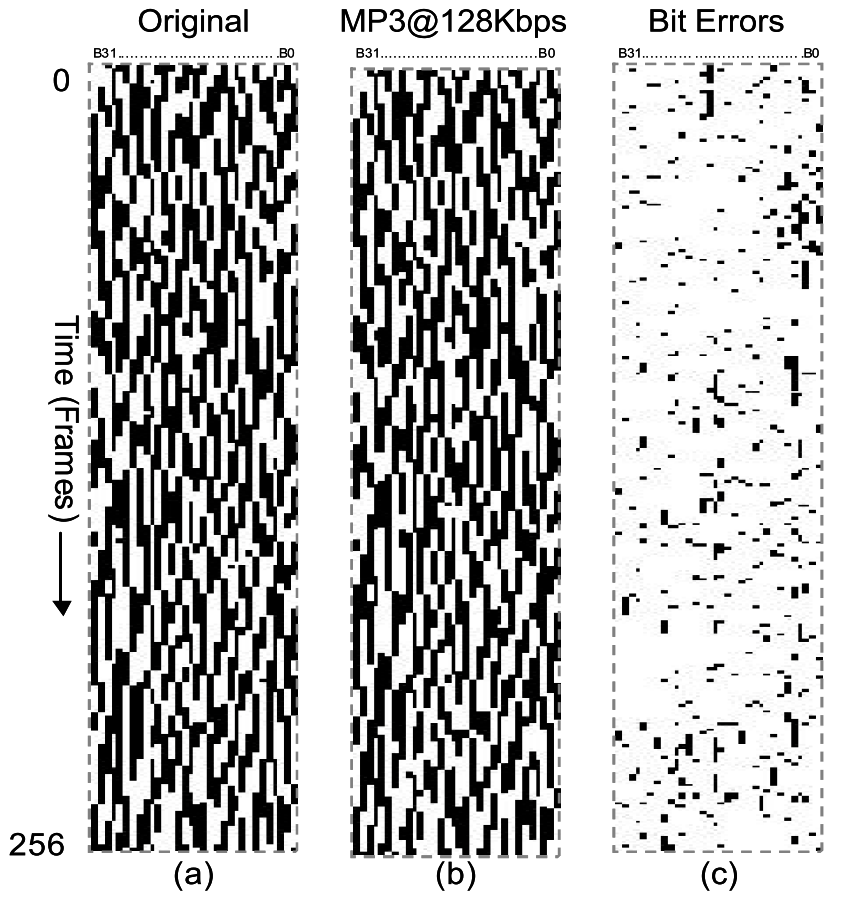
\includegraphics[scale=.25]{graph/fingerprint_example}
            \end{figure}
            \vspace{-10mm}plot from \footfullcite{haitsma_highly_2002}
        \end{frame}
        
        \begin{frame}{audio fingerprinting}{system example: philips identification 1/3}
            \begin{itemize}
                \item	\textbf{database}
                    \begin{itemize}
                        \item	contains all subfingerprints for all songs
                        \item<2->	previous example database: $25$ billion subfingerprints
                        \bigskip
                    \end{itemize}
                \item<3->	\textbf{problem}
                    \begin{itemize}
                        \item how to identify fingerprint efficiently?
                    \end{itemize}
            \end{itemize}
        \end{frame}
        
        \begin{frame}{audio fingerprinting}{system example: philips identification 2/3}
            \begin{itemize}
                \item \textbf{simple system}:
                    \begin{enumerate}
                        \item	create lookup table with all possible subfingerprints ($2^{32}$) pointing to occurrences
                        \bigskip
                        \item<2->	assume at least one of the extracted $256$ subfingerprints is error-free\\
                        \item<2->[$\Rightarrow$] only entries listed at $256$ positions of the table have to be checked
                        \bigskip
                        \item<3->	compute \textit{Hamming} distance between extracted fingerprint and candidates
                    \end{enumerate}
            \end{itemize}
        \end{frame}
        
        \begin{frame}{audio fingerprinting}{system example: philips identification 3/3}
            \begin{itemize}
                \item \textbf{variant 1}: 
                    \begin{itemize}
                        \item	allow \textit{one} bit error 
                        \item<2->[$\Rightarrow$] workload increase by factor $33$
                     \end{itemize}
               \bigskip
                \item<3-> \textbf{variant 2}: 
                    \begin{itemize}
                        \item<3->	introduce concept of bit error probability into fingerprint extraction
                            \begin{itemize}
                                \item	small energy difference $\rightarrow$ high error probability
                                \item	large energy difference $\rightarrow$ low error probability
                            \end{itemize}
                        \bigskip
                        \item<4->	rank bits per subfingerprint by error probability and check only for bit errors at likely positions
                    \end{itemize}
            \end{itemize}
        \end{frame}

     \section{shazam}   
        \begin{frame}{audio fingerprinting}{other systems: shazam}
            \vspace{-3mm}
            \begin{figure}
                \centering
                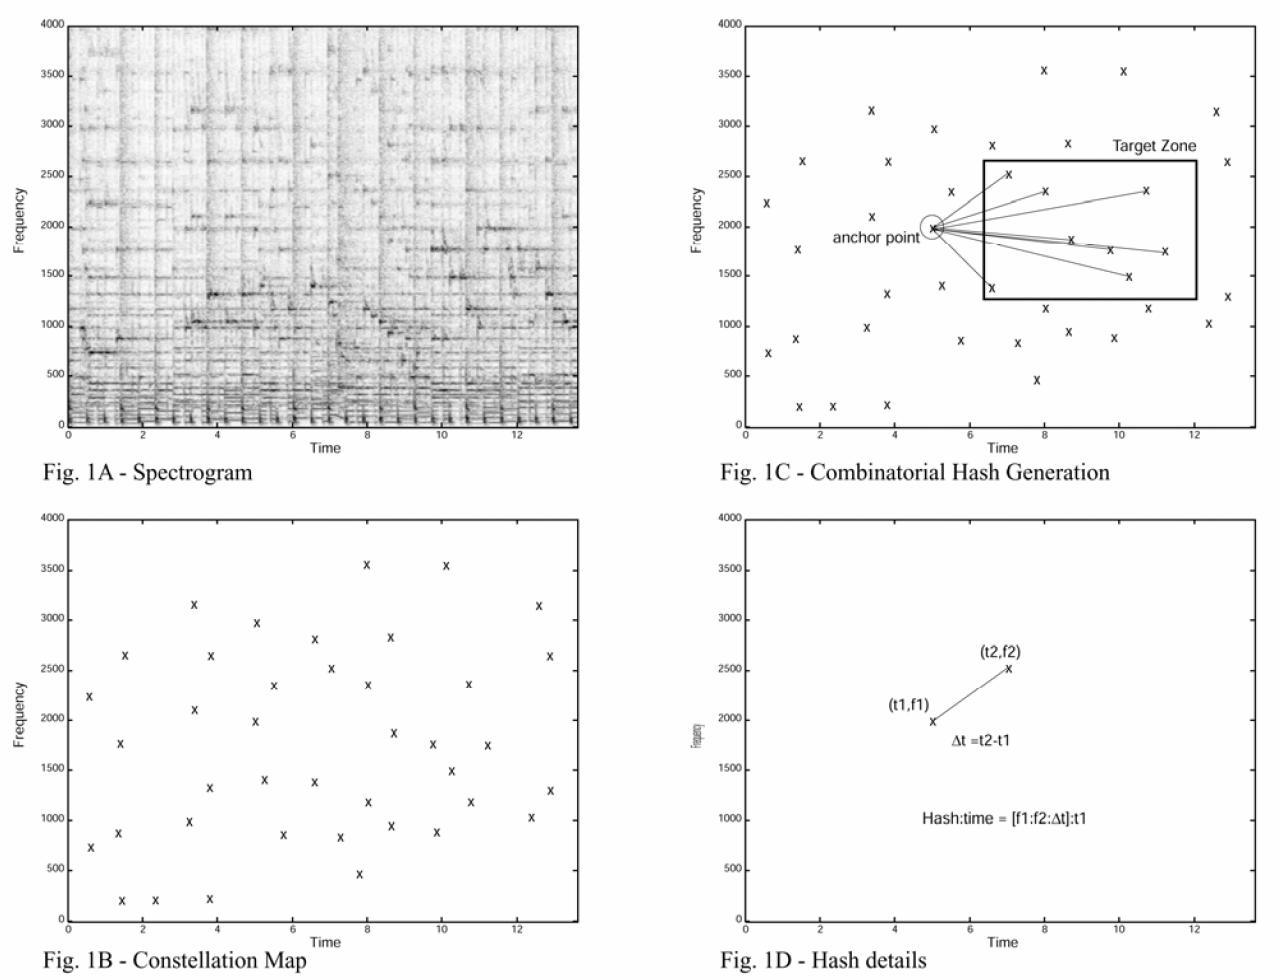
\includegraphics[scale=.23]{graph/fingerprint_shazaam}
            \end{figure}
            \vspace{-5mm}
            plot from \footfullcite{wang_industrial_2003}
            
        \end{frame}
    
    \section{summary}
        \begin{frame}{summary}{lecture content}
            \begin{itemize}
                \item   \textbf{audio fingerprinting}
                    \begin{itemize}
                        \item   represent recording with compact, robust, and unique fingerprint
                        \item   allow efficient matching of this fingerprint with database
                    \end{itemize}
                \bigskip
                \item   \textbf{often confused with other tasks}
                    \begin{enumerate}
                        \item   audio watermarking
                        \item   cover song detection
                    \end{enumerate}
            \end{itemize}
            \inserticon{summary}
        \end{frame}
\end{document}
